% !TEX TS-program = pdflatex
% !TEX encoding = UTF-8 Unicode

% This is a simple template for a LaTeX document using the ``article'' class.
% See ``book'', ``report'', ``letter'' for other types of document.

\documentclass[11pt]{article} % use larger type; default would be 10pt

\usepackage[utf8]{inputenc} % set input encoding (not needed with XeLaTeX)

%%% Examples of Article customizations
% These packages are optional, depending whether you want the features they provide.
% See the LaTeX Companion or other references for full information.

%%% PAGE DIMENSIONS
\usepackage{geometry} % to change the page dimensions
\geometry{a4paper} % or letterpaper (US) or a5paper or....
\geometry{margin=1in} % for example, change the margins to 2 inches all round
% \geometry{landscape} % set up the page for landscape
%   read geometry.pdf for detailed page layout information

\usepackage{graphicx} % support the \includegraphics command and options

% \usepackage[parfill]{parskip} % Activate to begin paragraphs with an empty line rather than an indent

%%% PACKAGES
\usepackage{booktabs} % for much better looking tables
\usepackage{array} % for better arrays (eg matrices) in maths
\usepackage{paralist} % very flexible & customisable lists (eg. enumerate/itemize, etc.)
\usepackage{verbatim} % adds environment for commenting out blocks of text & for better verbatim
\usepackage{subfig} % make it possible to include more than one captioned figure/table in a single float
% These packages are all incorporated in the memoir class to one degree or another...
\usepackage{enumitem}
\usepackage{amsmath}

% para los cuadritos en links
%\usepackage[linkbordercolor={0 0 1}, citebordercolor={0 1 0}, urlbordercolor={1 0 0}]{hyperref}
\usepackage[colorlinks=true, linkcolor=black, citecolor=green, urlcolor=red]{hyperref} % solo resalta
\usepackage[spanish]{babel}



%%% HEADERS & FOOTERS
\usepackage{fancyhdr} % This should be set AFTER setting up the page geometry
\pagestyle{fancy} % options: empty , plain , fancy
\renewcommand{\headrulewidth}{0pt} % customise the layout...
\lhead{}\chead{}\rhead{}
\lfoot{}\cfoot{\thepage}\rfoot{}

%%% SECTION TITLE APPEARANCE
\usepackage{sectsty}
\allsectionsfont{\sffamily\mdseries\upshape} % (See the fntguide.pdf for font help)
% (This matches ConTeXt defaults)

%%% ToC (table of contents) APPEARANCE
\usepackage[nottoc,notlof,notlot]{tocbibind} % Put the bibliography in the ToC
\usepackage[titles,subfigure]{tocloft} % Alter the style of the Table of Contents
\renewcommand{\cftsecfont}{\rmfamily\mdseries\upshape}
\renewcommand{\cftsecpagefont}{\rmfamily\mdseries\upshape} % No bold!

%%% END Article customizations

%%% The ``real'' document content comes below...

\title{Trabajo práctico 1\\ Redes Neuronales y Aprendizaje Profundo}
\author{Ignacio Ezequiel Cavicchioli\\Padrón 109428\\icavicchioli@fi.uba.ar}
\date{10/9/2025} % Activate to display a given date or no date (if empty),
         % otherwise the current date is printed



\begin{document}
\maketitle

\tableofcontents



\section{Introducción}

Este documento presenta el desarrollo de las consignas del trabajo práctico N°2 de la materia de \textbf{Redes Neuronales y Aprendizaje Profundo}.  El código correspondiente fue realizado en  \textit{Jupyter notebooks}, \textit{Python}, adjuntados a la entrega en formato PDF. Toda imagen o implementación requeridas para el análisis se explicitarán en el presente archivo, por lo que la lectura del código en sí queda a discreción del lector. La teoría relevante será presentada y discutida en la sección pertinente.


\newpage

\section{Ejercicio 1}

\subsection{Consignas}

Implemente un perceptrón simple que aprenda la función lógica AND y la función lógica OR, de 2 y de 4 entradas. Muestre la evolución del error durante el entrenamiento. Para el caso de 2 dimensiones, grafique la recta discriminadora y todos los vectores de entrada de la red.

\subsection{Desarrollo}


\begin{figure}[h!]
	\centering
	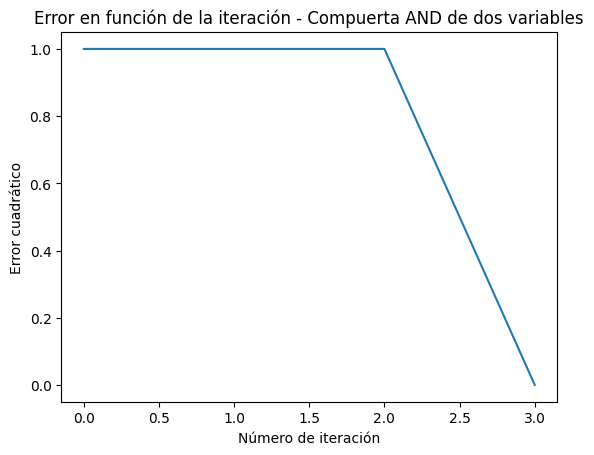
\includegraphics[width=0.7\linewidth]{../imgs/ej1/AND2err}
	\caption[]{Error de entrenamiento en el tiempo para compuerta AND de 2 entradas}
	\label{fig:and2err}
\end{figure}


\begin{figure}[h!]
	\centering
	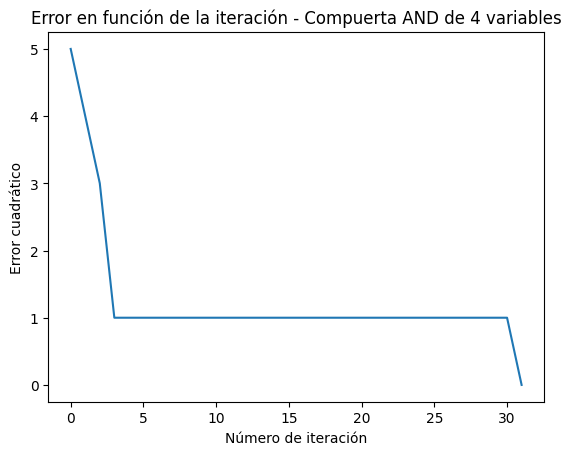
\includegraphics[width=0.7\linewidth]{../imgs/ej1/AND4}
	\caption[]{Error de entrenamiento en el tiempo para compuerta AND de 4 entradas}
	\label{fig:and4}
\end{figure}



\begin{figure}[h!]
	\centering
	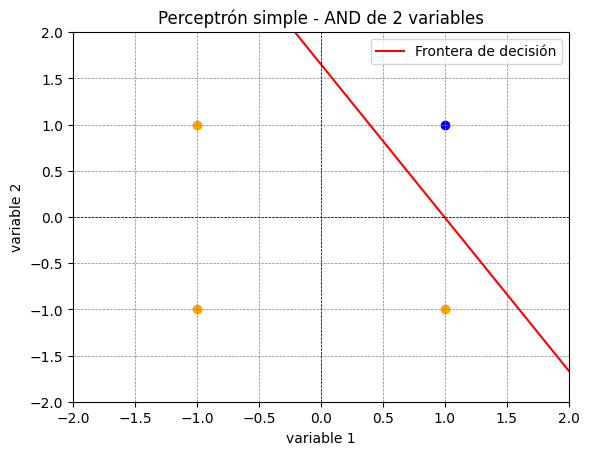
\includegraphics[width=0.7\linewidth]{../imgs/ej1/ANDFRONT}
	\caption[]{Frontera encontrada para compuerta AND de 2 entradas}
	\label{fig:frontAND}
\end{figure}

\begin{figure}[h!]
	\centering
	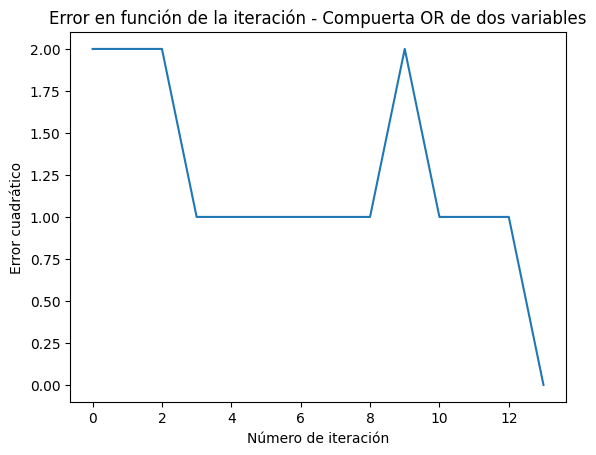
\includegraphics[width=0.7\linewidth]{../imgs/ej1/OR2err}
	\caption[]{Error de entrenamiento en el tiempo para compuerta OR de 2 entradas}
	\label{fig:or2err}
\end{figure}

\begin{figure}[h!]
	\centering
	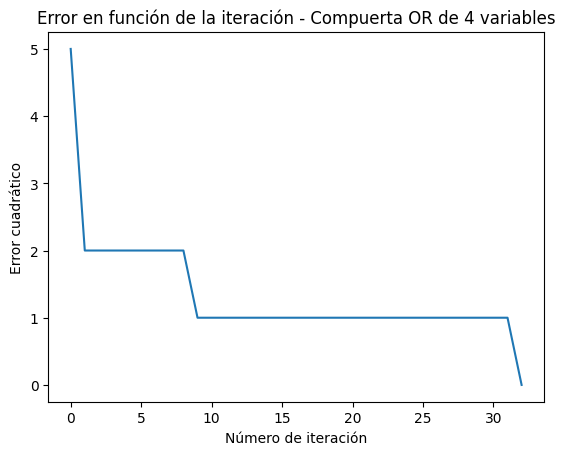
\includegraphics[width=0.7\linewidth]{../imgs/ej1/OR4}
	\caption[]{Error de entrenamiento en el tiempo para compuerta OR de 4 entradas}
	\label{fig:or4}
\end{figure}

\begin{figure}[h!]
	\centering
	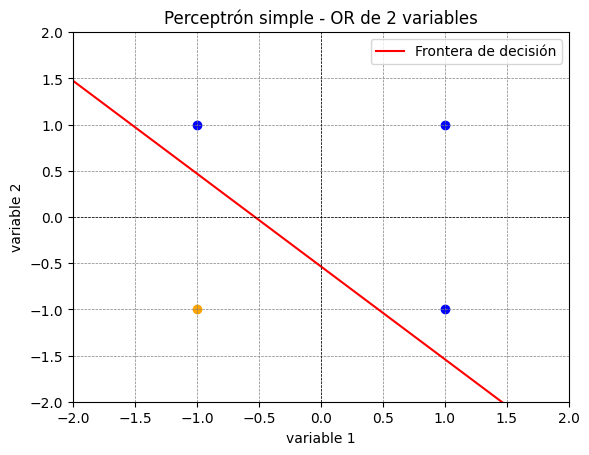
\includegraphics[width=0.7\linewidth]{../imgs/ej1/ORFRONT}
	\caption[]{Frontera encontrada para compuerta OR de 2 entradas}
	\label{fig:orfront}
\end{figure}


\subsection{Análisis}

\section{Ejercicio 2}

\subsection{Consignas}

Determine numéricamente cómo varía la capacidad del perceptrón simple en función del número de patrones enseñados.


\subsection{Desarrollo}


\begin{figure}[h!]
	\centering
	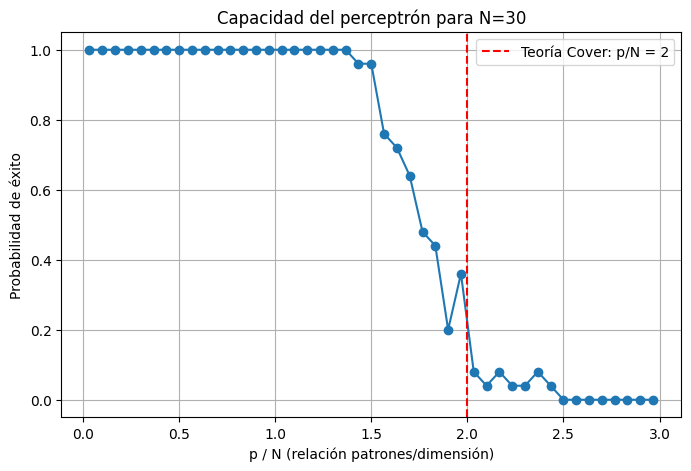
\includegraphics[width=0.7\linewidth]{../imgs/ej2/capacidad}
	\caption[]{Ensayo de capacidad $N=30$}
	\label{fig:capacidad}
\end{figure}


\subsection{Análisis}

\section{Ejercicio 3}

\subsection{Consignas}

Implemente un perceptrón multicapa que aprenda la función lógica XOR de 2 y de 4 entradas (utilizando el algoritmo Backpropagation y actualizando en batch). Muestre cómo evoluciona el error durante el entrenamiento.

\subsection{Desarrollo}
\begin{figure}
	\centering
	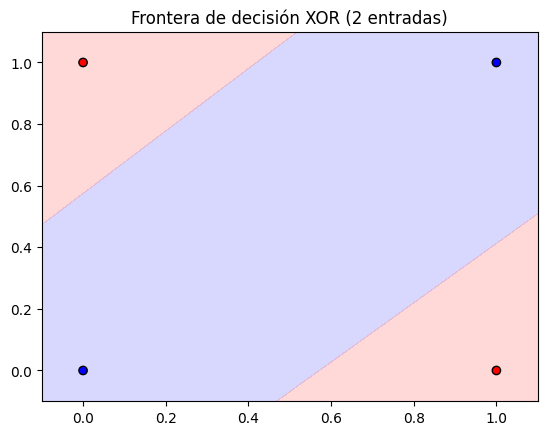
\includegraphics[width=0.7\linewidth]{imgs/ej3_frontera_xor}
	\caption{}
	\label{fig:ej3fronteraxor}
\end{figure}


\begin{figure}
	\centering
	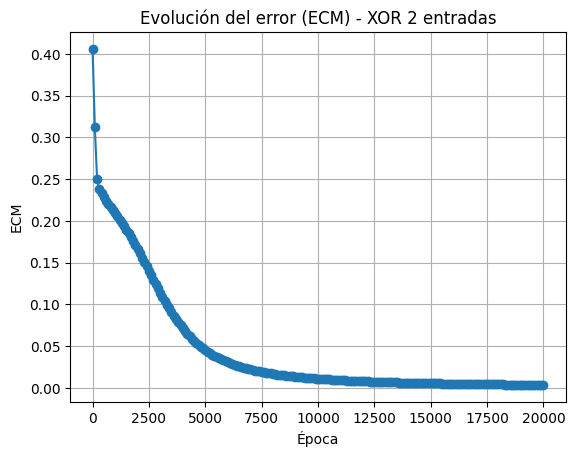
\includegraphics[width=0.7\linewidth]{imgs/ej3__error_xor2}
	\caption{}
	\label{fig:ej3errorxor2}
\end{figure}

\begin{figure}
	\centering
	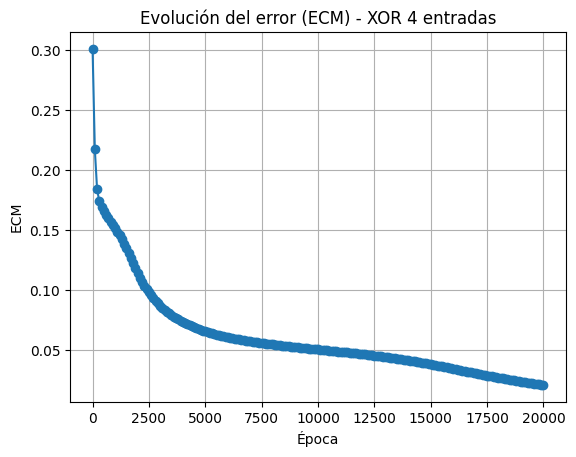
\includegraphics[width=0.7\linewidth]{imgs/ej3__error_xor4}
	\caption{}
	\label{fig:ej3errorxor4}
\end{figure}


\subsection{Análisis}


\section{Ejercicio 4}

\subsection{Consignas}

a - Implemente una red con aprendizaje Backpropagation que aprenda la siguiente función:
$$
f (x , y , z)= \sin(x)+\cos(y)+z
$$

donde: $x$ e $y$ $\in [0,2 \pi]$ y $z \in [-1,1]$.

Para ello construya un conjunto de datos de entrenamiento y un conjunto de evaluación. Muestre la evolución del error de entrenamiento y de evaluación en función de las épocas de entrenamiento.

b - Estudie la evolución de los errores durante el entrenamiento de una red con una capa oculta de 30 neuronas cuando el conjunto de entrenamiento contiene 40 muestras. ¿Que ocurre si el minibatch tiene tamaño 40? ¿Y si tiene tamaño 1?

\subsection{Desarrollo}

\subsection{Análisis}






\section{Ejercicio 5}

\subsection{Consignas}

Siguiendo el trabajo de Hinton y Salakhutdinov (2006), entrene una máquina restringida de Boltzmann con imágenes de la base de datos MNIST. Muestre el error de reconstrucción durante el entrenamiento, y ejemplos de cada uno de los dígitos reconstruidos.
\subsection{Desarrollo}

\subsection{Análisis}


\section{Ejercicio 6}

\subsection{Consignas}

Entrene una red convolucional para clasificar las imágenes de la base de datos MNIST.
¿Cuál es la red convolucional más pequeña que puede conseguir con una exactitud de al menos 90\% en el conjunto de evaluación? ¿Cuál es el perceptrón multicapa más pequeño que puede conseguir con la misma exactitud?

\subsection{Desarrollo}

\subsection{Análisis}





\section{Conclusiones}

\end{document}
